\documentclass[11pt, oneside, fullpage, doublespace]{article}
\usepackage{geometry}                		% See geometry.pdf to learn the layout options. There are lots.
\geometry{letterpaper}                   		% ... or a4paper or a5paper or ... 
%\geometry{landscape}                		% Activate for for rotated page geometry
%\usepackage[parfill]{parskip}    		% Activate to begin paragraphs with an empty line rather than an indent
\usepackage{graphicx}				% Use pdf, png, jpg, or eps� with pdflatex; use eps in DVI mode
								% TeX will automatically convert eps --> pdf in pdflatex		
\usepackage{amssymb}
\usepackage{hyperref}
\usepackage{color}

\usepackage{setspace}
\setstretch{1.5}
\usepackage{enumerate}
\usepackage{paralist}


% Code formatting
\usepackage{listings}
\usepackage{color}
\definecolor{mygreen}{rgb}{0,0.6,0}
\definecolor{mygray}{rgb}{0.5,0.5,0.5}
\definecolor{mymauve}{rgb}{0.58,0,0.82}
\lstset{ %
  backgroundcolor=\color{white},   % choose the background color
  basicstyle=\footnotesize\ttfamily,        % size of fonts used for the code
  breaklines=true,                 % automatic line breaking only at whitespace
  captionpos=b,                    % sets the caption-position to bottom
  commentstyle=\color{mygreen},    % comment style
  escapeinside={\%*}{*)},          % if you want to add LaTeX within your code
  keywordstyle=\color{blue},       % keyword style
  stringstyle=\color{mymauve},     % string literal style
}



\title{Wireless Automobile Detection, License Plate Processing, and Data Availability Network}
\author{Kevin Emery, Santiago Gonzalez, Brandon Rodriguez, Taylor Sallee\\ \emph{Undergraduates, EECS Department, Colorado School of Mines}}
\date{April 28, 2014}


\begin{document}
\maketitle

\begin{abstract}
{\color{red}\textbf{NOT COMPLETE}}
This proposal describes a parking lot monitoring system to be used at the Colorado School of Mines (CSM). The system will help campus members enjoy a better parking experience by spending less time trying to find open lots. This is a semester project for the Computer Science graduate course \emph{Wireless Sensor Networks}, taught by Dr. Tracy Camp at CSM. The proposed work will be an extension of a project started by campus computing group ACMx, which uses a wireless sensor network to track the number of cars in specific parking lots. The system will extend the ACMx project by adding components to the sensor network that record the license plate numbers of cars as they enter and exit lots. The information gathered by the sensor network will be displayed on a website that will allow users to survey the state of the lots before arriving, allowing them to make informed parking decisions. The website will also be the result of collaboration between the authors of this proposal and the ACMx group. The proposal provides some background information, describes the proposed system and its components, and discusses implementation strategies. The goal of the project is a real-world deployment on the CSM campus by May 2014.
\end{abstract}


\section{Introduction}
{\color{red}\textbf{NOT COMPLETE}}
The parking lots at the Colorado School of Mines (CSM) can be a source of frustration for students and faculty members. Because space on campus is limited, the lots are often unable to accommodate everyone who needs to use them. Students need to choose a lot before they go to class; however, knowing which lots have free spaces usually requires driving through the lots looking for a space. The extra time spent searching one or many lots can make students or faculty late for class. If campus members could find out which lots had available spaces before they arrived, much time and frustration could be saved. The goal of this project is to design and deploy a working parking lot monitoring system that will be the first step towards a better parking experience on the CSM campus. The system will keep track of both the number of vehicles in a parking lot and the license plate numbers of those vehicles. The information will be available online to system administrators and CSM campus members. There are two main parts to this project:

\begin{enumerate}
\item Parking lot capacity monitoring
\item License plate detection and monitoring
\end{enumerate}

The idea behind the first part is that a student can get on their smartphone, tablet, or laptop before heading to class, see a nicely-formatted list/map of the lots on campus, and decide where to park based on how full each lot is. Administrators will monitor the information and make sure it is correct, updating the web application as needed with new statistics, lists and maps as more lots are added to the system. The Association for Computing Machinery group (ACMx) at CSM has already started working on a system for monitoring lot capacities (see section 1.2). We will collaborate closely with the ACMx group, integrating our work with theirs to create and deploy a working system by the end of this semester (May 2014).

The second part of the project is motivated by a desire to test the feasibility of using the small Raspberry Pi Linux computer as a platform for capturing and processing images of license plates. Because the Raspberry Pi is inexpensive (\$25-\$35 depending on model), it could be useful in a wide variety of applications that require accurate license plate recognition. For now our web application will simply list the license plate numbers for site administrators to view, but we envision that this monitoring system may eventually be used by the campus parking department to detect when vehicles have entered lots without parking passes.

The goal of this project is to work with the ACMx group to create and deploy the system in two parking lots on campus by the end of the semester. See section 2.7 for information about the deployment. The system itself will consist of several subsystems, which are described in detail in section 2.

\section{Related Work {\color{red}\textbf{NOT COMPLETE}} }
The ACMx group at CSM has designed a system named SmartLots to track the number of vehicles in a parking lot. Their system is a wireless sensor network consisting of sensor nodes and a central base station. The sensor nodes are based on the Arduino Fio microcontroller platform equipped with triaxial magnetometers and XBee Pro radios. The base station is a Raspberry Pi connected to the internet via Ethernet. The information collected by the sensor nodes is transmitted to the base station and forwarded to a server running a small web application. The system is described in \cite{stillwell2013} and \cite{parkingWiki}. \cite{stillwell2013} describes an implementation of a system to detect automobiles entering and exiting a parking lot using the Arduino Fio and the Raspberry Pi. This system uses the IEEE 802.15.4 communications standard to communicate automobile detection data from the sensor nodes to the base station. \cite{parkingWiki} describes the ongoing status of the ACMx project. At the time of writing, the ACMx team has created a website that will display the status of the CTLM upper and lower lots once the monitoring system has been deployed. \cite{parkingWiki} is updated periodically with new information regarding project progress. The project described in this paper augments and extends the ACMx project while collaborating with Stillwell (ACMx president and coauthor of \cite{stillwell2013}).

\section{Project Overview and Methods {\color{red}\textbf{NOT COMPLETE}} }
\begin{figure}
\begin{center}
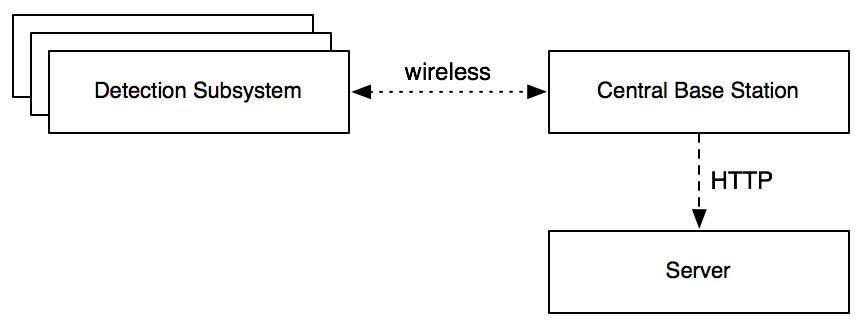
\includegraphics[width=4.5in]{architecture}
\end{center}
\caption{Overall System Architecture}
\label{fig:system}
\end{figure}
This project is partially an extension of the ACMx SmartLots project. The system consists of several components, each of which will is either an extension of a current SmartLots system or an entirely new subsystem that has been integrated into the existing system. Figure \ref{fig:system} shows the overall architecture of our system. The system relies on three main components:
\begin{enumerate}
\item Detection Subsystem,
\item Central Base Station, and
\item Server.
\end{enumerate}

The detection subsystem consists of a small number of sensor nodes, placed strategically at parking lot entrances. Each sensor node will contain an Arduino Fio equipped with a triaxial magnetometer that will be used to detect when a car passes the sensor. The work to determine the hardware configuration and software for the Arduino Fios has already been done by the ACMx group in \cite{stillwell2013}. Each sensing node is also equipped with a Raspberry Pi single-board computer and a 5 megapixel camera, which take photographs of the license plates of cars as they pass by. When a car passes a sensor node, the magnetometer will detect the car, and the Arduino Fio will send a hardware interrupt to the Raspberry Pi, running a Python script so that the camera can take a picture of the license plate. These images are then run through an OpenCV Python program to reduce the size of the image, through downscaling, cropping, and compression algorithms.

A Raspberry Pi operates as a central base station that receives automobile detection and status data from every sensor node, via transmission from the XBee radios attached to the sensor nodes. The base station Raspberry Pi will be centrally located in a nearby building with internet connectivity. The base station utilizes its network connection to forward the data to the ACMx server.

The server runs a PHP web application with an RESTful HTTP interface that both receives the data from the base station and routes it to the correct part of the application (database, image processor, etc.). This interface will be the method of communication between the server and the base station. When data is received from the base station, the application processes it, stores it in a MySQL database, and displays it appropriately on a user-facing website. An administrator website also exists that provides direct access to license plate data and car counts.

{\color{red}\textbf{NOT COMPLETE}} The following sections describe the architecture and function of each of the aforementioned subsystems in detail. The detection subsystem is broken up into two parts: Automobile Detection (section 2.2) and License Plate Image Acquisition (section 2.3). The server subsystem is also broken into two parts: Server Processing (section 2.5) and Web Application (section 2.6). Lastly, section 2.4 discusses the Central Base Station.

\subsection{Automobile Detection}
{\color{red}\textbf{NOT COMPLETE}}
The automobile detection subsystem will provide a means for detecting ingress and egress of vehicles from a parking lot. This subsystem is to be placed on the side of the road next to each parking lot entrance and exit. Automobiles will be detected using a magnetometer which perceives the induced change in the local magnetic field as the metallic structure of the vehicle passes by, as described in \cite{stillwell2013}. The automobile detection subsystem will be based around the commercially available Arduino Fio 16-bit  platform which utilizes the ubiquitous Atmel ATMEGA328p microcontroller. When an automobile is detected by the Arduino Fio, a packet will be sent through the onboard XBee radio to the central base station (described in section 2.4). The packet will  contain the direction of the passing vehicle. At the time of detection, a hardware interrupt will also be sent to the license plate recognition system to awaken it from sleep mode.

\begin{figure}
\begin{center}
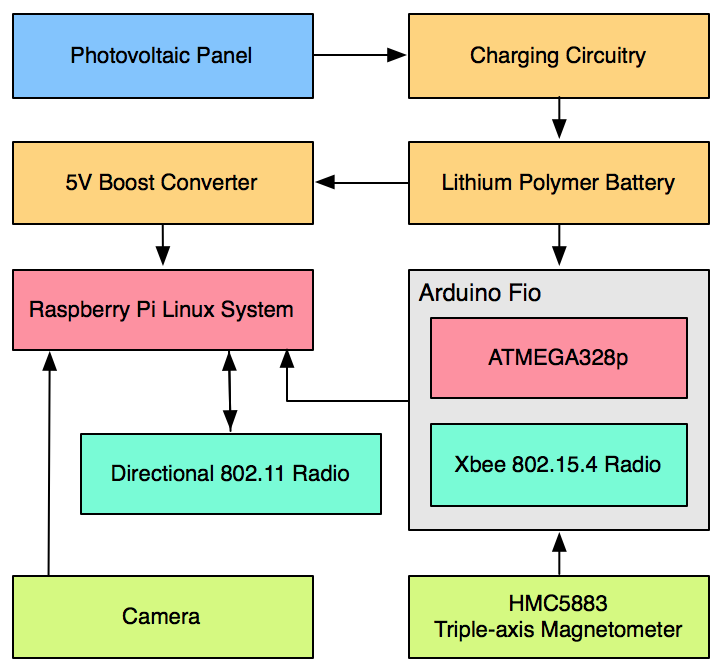
\includegraphics[width=3.5in]{autodetection}
\end{center}
\caption{Automobile Detection Subsystem Architecture}
\label{fig:autodetect}
\end{figure}

The hardware to be used for automobile detection will be contained in the same enclosure as the license plate image acquisition hardware for simplicity. Both components will share a unified power supply based on a high-capacity lithium polymer battery, which will be charged by a relatively small photovoltaic panel as seen in Figure~\ref{fig:autodetect}. A 5V boost converter will be required to interface with the Acquisition Raspberry Pi since the lithium polymer batteries only provide 3.7V.

The use of a magnetometer ensures that automobiles and other roadway vehicles such as motorcycles are detected, while pedestrians and particulate deposits, such as snow, are ignored. As mentioned in \cite{stillwell2013}, the automobile detection subsystem shall use the commercially available HMC5883 triaxial magnetometer as it provides an adequate balance of sensitivity and low power consumption.

\begin{figure}
\begin{center}
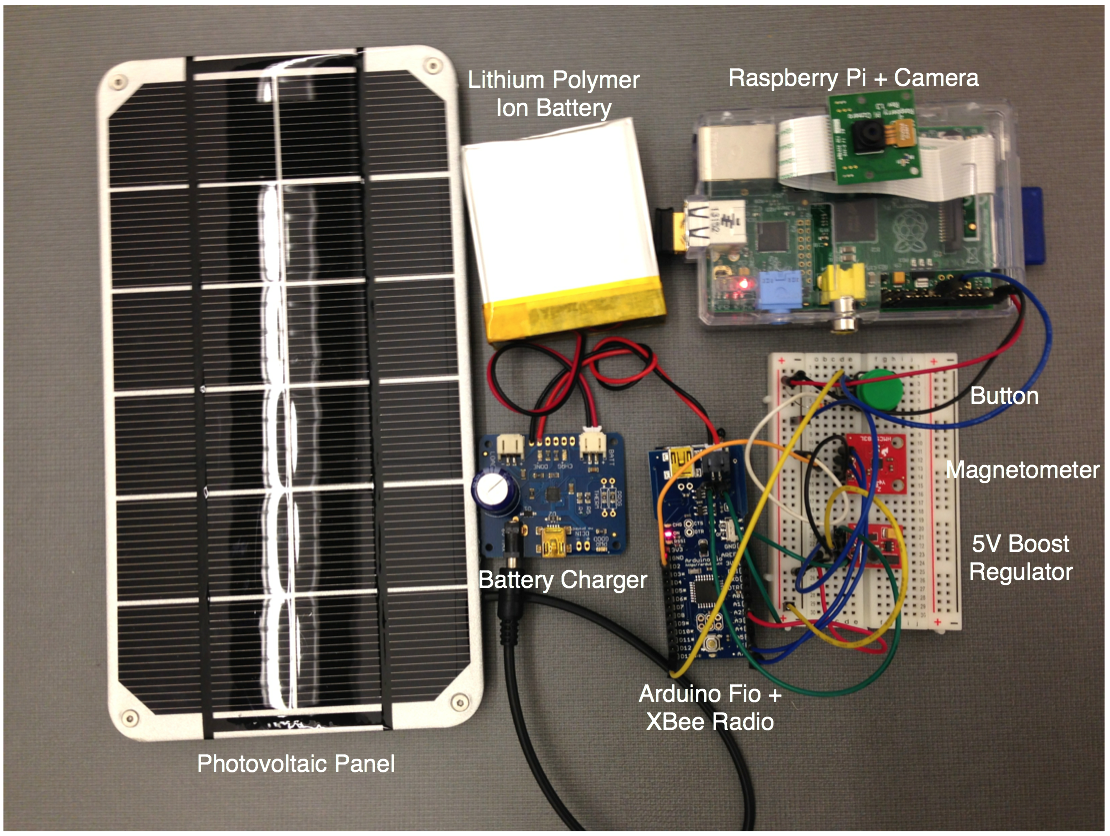
\includegraphics[width=4.5in]{sensornode}
\end{center}
\caption{Automobile Detection Node Hardware}
\label{fig:autodetecthardware}
\end{figure}

\subsubsection{Tests and Analyses}
{\color{red}\textbf{NOT COMPLETE}}
Because the ACMx group has already written the necessary software and designed a working configuration for detecting vehicles with the Arduino Fios, the bulk of our work on the automobile detection subsystem will involve a variety of tests and analyses to ensure system and data integrity. Power consumption analyses will be conducted on the automobile detection and license plate image acquisition subsystem to identify power usage per main component (Figure~\ref{fig:autodetect}) while the mote is in different states, such as sleeping and detecting vehicles. Such an analysis will allow us to allocate how much time the mote is allowed to spend in each state and determine the required lithium polymer battery capacity.

Analyses will also be performed on the timing of different actions within the network, including:
\begin{itemize}
\item Automobile detection lag
\item Imaging of vehicle
\item License plate recognition and extraction
\item Packet transmission
\end{itemize}
This will help determine whether certain portions of the image data processing may need to be performed on a server and whether it would be feasible to funnel the image data through the XBee instead of a dedicated directional IEEE 802.11 system.

The efficacy of the automobile detection subsystem will also be evaluated through several tests. A variety of different sized vehicles will be passed through the system at different velocities to ensure high detection accuracy. We will also analyze the end results of deployment after a certain period of time, to determine how often the automobile count needs to be reconciled.


\subsection{License Plate Image Acquisition}
{\color{red}\textbf{NOT COMPLETE}}
Once the Acquisition Raspberry Pi receives the interrupt from the vehicle detection Arduino Fio, it will begin the process of obtaining a picture of the vehicle's license plate. This procedure will be separated into two separate sections: image acquisition and license plate detection.

\subsubsection{Image Acquisition}
{\color{red}\textbf{NOT COMPLETE}}
While the automobile detection subsystem correctly identifies when a vehicle enters the lot, the image acquisition subsystem will be responsible for determining when to capture a picture of that car in order to optimize the quality of the license plate image. The timing difference between when the Raspberry Pi receives the interrupt and when it actually captures the picture will initially be determined experimentally using the average speed at which cars enter the parking lot. As the project progresses, this timing will be fine-tuned in order to capture the optimal image every time. The goal of this subsystem is to only take one picture to capture the license plate, so as to minimize capture time and power consumption.

\subsubsection{License Plate Detection}
{\color{red}\textbf{NOT COMPLETE}}
Once the image has been captured, the Raspberry Pi will then focus on detecting the license plate in the image and cropping the image to only include the license plate. This will be done in order to minimize the size of the transmission and the power required for that transmission. In order to detect the location of the license plate within the larger image, a detection algorithm needs to be applied.

The location of the license plates will be detected on the acquisition Raspberry Pi using the OpenCV (Open Source Computer Vision Library) API \cite{openCV}, which provides many different algorithms that can be used for image detection and shape recognition. This particular API was chosen for both its ease of use and widespread cross-compatibility; it has interfaces for development in C, C++, Python, Java, and MATLAB, and supports all major operating systems (including distributions of Linux such as Raspbian). Because OpenCV is used across the industry for image processing, we are confident that it will meet our needs.

Once the OpenCV software has detected the license plate, the image will then be cropped as needed until all that remains in the image is the license plate from the car that is entering the lot. That image will then be sent to the central base station via an XBee radio transmission.

\subsection{Central Base Station}
{\color{red}\textbf{NOT COMPLETE}}
\begin{figure}
\begin{center}
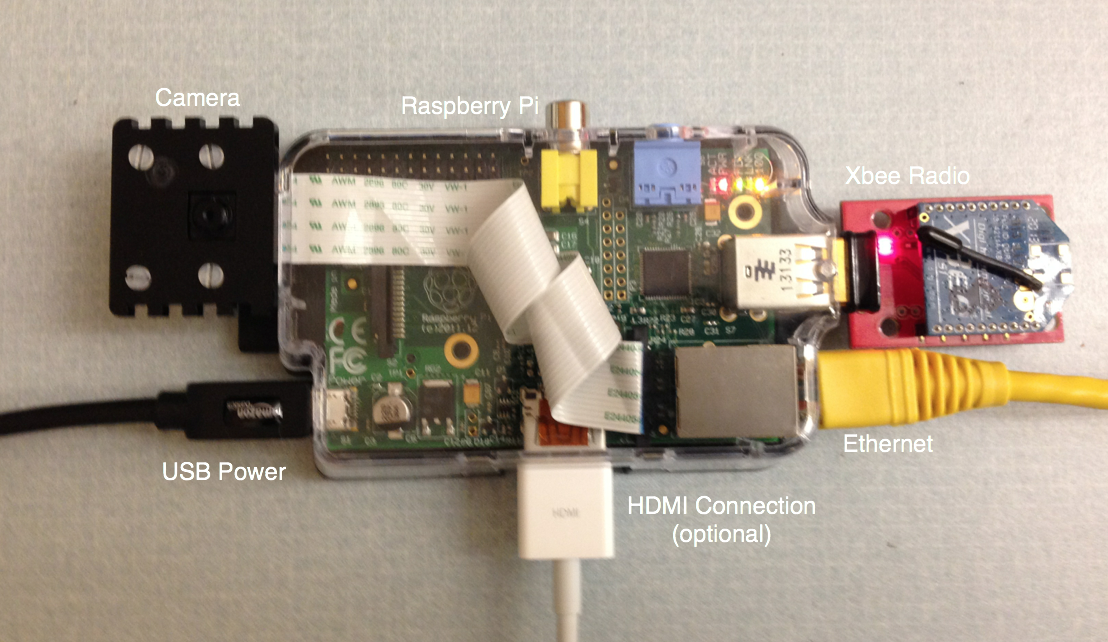
\includegraphics[width=4.5in]{basestation}
\end{center}
\caption{Central Base Station Hardware}
\label{fig:basestation}
\end{figure}
The central base station will be the point of contact between the sensor network and the server. The data gathered by the Arduino Fio and Raspberry Pi sensors will be routed to the base station via XBee radios. The base station, which will itself be a Raspberry Pi, will forward the data to the ACMx server using HTTP requests. Forwarding data is the main function of the base station. The base station will run the Raspbian operating system \cite{raspbian}, a lightweight version of Linux. Raspbian is optimized for the Raspberry Pi, so writing shell scripts that will take care of forwarding the data via HTTP to the server will be an easily achievable task. A second function of the base station will be to take periodic overhead photos of the parking lots to help reconcile the sensed data with the actual state of the lots. System administrators will be able to look at the photos to see if the number of cars reported in the lot by the sensors is correct, and fix any errors. See section 2.6 for more detailed information about the error correction functionality of the web application.


\subsection{Server Processing}
{\color{red}\textbf{NOT COMPLETE}}
Once an image has been captured by an Acquisition Raspberry Pi it is transmitted via the XBee radio to the base station Raspberry Pi where it is uploaded online via an Ethernet connection. The REST route that the image is posted serves several purposes. First, it authenticates the sender by checking for a username and password. The script then timestamps the image and saves it to a directory on the server not directly accessible from the web. Lastly, the script calls a function to invoke two different automatic license plate recognition (ALPR) programs and store the resulting character extraction to a MySQL database.

\subsubsection{ALPR Literature Survey}
{\color{red}\textbf{NOT COMPLETE}}
License plate extraction algorithms have been developed, implemented, and critiqued in the academic community. For use in our project, we needed to find an implemented ALPR algorithm capable of running in a Linux environment (on the server) or a cloud service that would allow for reliable character recognition from license images.

Much of the research done on ALPR technology is less concerned with implementation and more interested in algorithmic advances. License plate recognition relies heavily on manipulation of graphics files and computer vision - each fields of study in their own right. Despite the lack of detailed literature on implemented programs, we were still able to find papers that briefly mentioned two operational systems: OpenALPR and JavaANPR. Note that ALPR and ANPR are synonymous (some packages use the term 'number' plate recognition in place of 'license' plate recognition).

\emph{A. OpenALPR}

OpenALPR is a relatively new open source ALPR system that is built on top of OpenCV (a computer vision framework), and the Tesseract OCR engine. Initial commits to the source code were made in December, 2013. Using such a new program can be more risky than going with an established leader in the market, but we found that OpenALPR offered just the type of functionality we were looking for.

\emph{B. JavaANPR}

JavaANPR is an older program (published in 2007) that was created as part of a Bachelor's thesis at the Brno University of Technology in the Czech Republic. Stemming from an academic environment, JavaANPR has much more detailed documentation on the program and the algorithms implemented in the program than any other option surveyed (both academic and industrial). On the same token, development on the program seems to have stopped after the thesis was submitted, so the software has not seen updates in eight years. No software is perfect, and knowing that we would be using a program that is no longer being maintained is just one of the drawbacks we discovered about JavaANPR. The other main disadvantage of JavaANPR is that it was developed in Europe for European license plates. The source code would have to be correctly adapted in order to recognize North American plates, and the OCR engine would need to be trained for fonts used in America.

\emph{C. General ALPR Algorithm}

The two programs do share the same general algorithm for extracting license plates. First, the plate is identified using some means to isolate rectangles in the image (texture, color, boundaries, etc.). Once the bounding box containing the plate is found, segmentation begins to isolate each individual character on the license plate. Finally, these image representations of characters are mapped to their most likely plain text counterpart.

In general, ALPR systems only work for a specific geographic region they are "trained" for. For example, North American plates are a different size than European plates. Detection algorithms to identify a license plate in America would not work on an English car without modifications to the ALPR's configuration. Similarly, different states and countries use different fonts on their plates. In order to achieve maximum accuracy, you would need to collect hundreds of samples of the font and teach the program what those letters look like.


\subsubsection{ALPR Industry Survey}
{\color{red}\textbf{NOT COMPLETE}}
Many ALPR systems exist today for commercial and government purposes. Uses can range from cross-referencing address information with the DMV to bill users of toll roads to monitoring roadways for stolen cars or even measuring car speeds. Our team was able to contact two manufacturers of ALPR systems to learn more about their use in industry: Q-Free ASA and The 3M Company.

\emph{A. Q-Free ASA}

One commercial provider of ALPR software is Q-Free ASA, which is based out of the Netherlands. Q-Free is a top search result when querying for ALPR software. Their ALPR product, named Intrada, offers a cloud based solution where we are able to send the image of the license plate to their servers, and get back the plain text representation of the characters. One unique feature Intrada includes that we did not find in any other package surveyed is the ability to identify the state of origin of the license plate. Intrada does this by analyzing minor differences in fonts used across state borders.

Note that this feature is not the same as training OpenALPR or another system with a new font. In OpenALPR, new trained data helps increase accuracy in detection. As a user, you can ask OpenALPR to examine the probability of a "template match" to a specific font, but the software does not intelligently determine which font family it most closely matches. Intrada offers the simplest solution in terms of startup costs because there is no local software to configure on our machine.

\emph{B. The 3M Company}

E-470 uses high speed cameras to capture and extract license plate data in order to bill users of their toll road in the Denver Metro area. We reached out to the E-470 Public Highway Authority to inquire more about their deployment of sensors and ALPR software. Representatives informed us that their toll booths used an ALPR system developed by The 3M Company. Even though E-470 is using an ALPR which automatically detects the characters of a license plate, every image must be reviewed by a human operator before the driver is billed. In our project, we don't want a human operator to have to confirm each plate - we want to trust the ALPR to do its job.

After communicating with E-470, we contacted The 3M Company with regards to their ALPR software. A representative reached out and confirmed that they do offer an API to their program, allowing their technology to be built into other projects. Because we are creating a parking lot monitor system, and not just a license plate recognition system, an API is crucial so we can integrate the ALPR into our workflow. Unfortunately, our request for an educational use license for their ALPR was denied, as after reviewing our team's proposal 3M was worried we might try to commercialize our network. We were unable to learn more about their algorithm or API after that point.

\subsubsection{Selection of ALPR Programs}
{\color{red}\textbf{NOT COMPLETE}}
Our literature and industry surveys left us with three viable options for license plate recognition: OpenALPR, JavaANPR, and Q-Free's Intrada ALPR. Of those three, only OpenALPR was ready to be integrated into our network. Intrada ALPR is a commercial service, so our ability to use it was dependent on Q-Free granting an educational use license to us for the semester. Lastly, JavaANPR would need to be modified to detect and recognize North American plates and fonts. JavaANPR also lacks additional information that both OpenALPR and Intrada ALPR provide such as execution time and confidence.

The goal of this project is to demonstrate a proof of concept network that is capable of monitoring parking lots and capturing license plate data. To stay aligned with this goal, and because of our unfamiliarity with graphical algorithms, we decided not to pursue using JavaANPR as a software solution for our network.

After reaching out to Q-Free with regards to using their Intrada service for the semester, we were referred to their Global Account Manager OEM Partners representative Marco Sinnema. Dr. Sinnema, on behalf of Q-Free, graciously granted our request to use their product free of charge for the spring 2014 semester.

Instead of choosing between two ALPR systems, we decided to integrate both platforms into our network to allow an ALPR comparison between the two tools, and offer better data integrity by checking if results from both systems (for the same photo) matched.

\subsubsection{Test Data Collection}
{\color{red}\textbf{NOT COMPLETE}}
In order to evaluate the ALPR platforms, we needed to collect test data. Both platforms were already trained to run North American license plates out-of-the-box, so the stage was set to process images for a comparison in performance. With our final deployment in mind, we also wanted to collect images from a variety of different angles and distances, as the resulting evaluation will help determine the best camera placement in the CTLM parking lot. To accurately test the ALPR programs for our project, the test images need to be taken with the same camera that would be used during deployment.

We loaded a special testing script written in Python onto a Raspberry Pi to accomplish this task. The script was programmed to wait for a hardware interrupt before taking an image. We wired a button via a breadboard to provide the hardware interrupt. Our team brought this Pi, camera, and button out to the CTLM parking lot and positioned it near where it would be deployed.

Once powered on, we had one teammate drive their car in and out of the parking lot multiple times. While he was driving, two other team members operated the camera and breadboard hardware to take images. Using the same license plate for this portion of our test data acquisition was intentional to lower the number of uncontrolled variables in gathering data.

Besides images of the same license plate, we also collected several images of nearby parked cars, as well as cars that entered or exited the CTLM parking lot during that time period. And because our system is to be deployed on a college campus, we also collected images from different states, as the population of nonresidents is much greater here than in neighboring small towns.

Overall, we were able to collect 56 images of seven different plates that contained recognizable numbers. Each image from the Raspberry Pi camera was about 3 megabytes in size in its uncompressed form. The Python script also specified that the camera should save in a JPEG (.jpg) format.

The data set, which we will now refer to as the \emph{Unaltered Data Set}, is the basis for all other data sets in this paper. That is, all other data sets are derived from these original, uncompressed images. 

\subsubsection{ALPR-Project Integration}
{\color{red}\textbf{NOT COMPLETE}}
Both OpenALPR and Intrada ALPR had to be integrated into our web application so they would run automatically without the need for human intervention. OpenALPR, because it is not a cloud service, needed to be installed locally on the ACMx server. The Intrada ALPR was much simpler because we were only interacting with the API.

\emph{A. OpenALPR}
{\color{red}\textbf{NOT COMPLETE}}
As stated in ??? LITERATURE SURVEY REFERENCE ???, OpenALPR is built on top of OpenCV, a computer vision library, and Tesseract OCR, an OCR engine. Tesseract OCR had additional dependencies that needed to be installed before it would compile.

We used Ubuntu's \verb+apt-get+ command to install almost all of Tesseract's dependency packages. Tesseract makes use of a recent version of an image processing software called Leptonica. Because the version used in Tesseract superseded the versions available in Ubuntu's repository, we had to download the source files for Leptonica and compile it from scratch.

After installing all the dependencies, we were finally able to compile Tesseract from its source files. Additionally, OpenCV came bundled with all of its dependencies, so we were able to build the OpenCV library rather effortlessly.

Once OpenCV and Tesseract were operational, compiling OpenALPR was a breeze. The entire process of installing all the dependencies and compiling everything (correctly) took a full working day. After installation, OpenALPR was able to start recognizing license plates immediately because it comes bundled with training data for both North American and European plates.

\emph{B. Intrada ALPR}
{\color{red}\textbf{NOT COMPLETE}}
Intrada ALPR uses the SOAP protocol for exchanging information. To create SOAP requests, we used the \verb+SoapClient+ class available in PHP to create, send, and receive the output of our request.

Intrada requires a username and password to process images. The SOAP API allows for the sending of the username and password as part of each request object for authentication. Then, Intrada runs their proprietary algorithm on its own servers before returning a result string back to our web application. The result string contains colon delimited fields that carry 
\begin{inparaenum}[\itshape a\upshape)]
\item the extracted license plate characters;
\item the confidence in the extraction;
\item the state of origin of the license plate;
\item the confidence in the state of origin;
\item coordinates of the boundary box of the detected license plate; and
\item the execution time for the specified image.
\end{inparaenum}

\subsubsection{ALPR Evaluation Environment}
The ALPR software is 



\subsubsection{Proposal part}
{\color{red}\textbf{NOT COMPLETE}}
Once an image has been determined to contain a license plate, it will be transmitted from the Acquisition Raspberry Pi to a server online via the base station Raspberry Pi. The server will then be responsible for using recognition software technology to extract the digits of the license plate from the image. Upon successful completion, the textual representation of the license plate will be stored in a database residing on the server to be later integrated into the front-facing web application.

The subsystem encapsulating server processing will require a review of recognition software and literature. There exists a market for Automatic License Plate Recognition (ALPR) software that relies on Optical Character Recognition (OCR) engines to extract characters. \cite{du2013} describes the various methods and features used to extract characters from a license plate. Once an ALPR solution is chosen, it will be necessary to collect a set of test data using the Acquisition Raspberry Pi to tune the workflow of character extraction.

\subsubsection{Considerations for ALPR Software}
{\color{red}\textbf{NOT COMPLETE}}
For the scope of this project, three ALPR solutions will be evaluated to determine which is the most suitable for our purposes. An ideal ALPR software needs to be currently maintained and capable of reading a license plate if it is skew in an image, taken in poor lighting conditions, and taken with low resolution.

Q-Free Intrada ALPR \cite{intrada2014} is a license plate recognition software that offers a C++ API, as well as a cloud-based service. Both the API and cloud-based service can be utilized from a Linux server. Q-Free's software is used in countries around the world for traffic management and toll collection. The wide-ranging geography of its use mean that Intrada ALPR is likely to be reliable and accurate for all types of license plates. Use of the Intrada suite is dependent on Q-Free granting an educational use license for this semester.

OpenALPR is another C++ library for use with both North American and European plates. This library relies upon two underlying technologies: OpenCV \cite{openCV} and Tesseract OCR (an OCR engine being developed and maintained by Google). The Tesseract OCR Tool is self-sufficient, and relies on included training data. \cite{patel2012} goes into greater detail how Tesseract extracts data from images. The open-source nature of this project make it appealing as it can be immediately integrated without needing to obtain an educational license first. Additionally, the last updates were pushed to the source repository in January. While it is desirable for the software we consider to be relatively up-to-date and maintained, this repository was started only four months ago (November, 2013). Use of such a young library may create a less stable solution than what is practical to work with throughout the course of the semester.

JavaANPR markets itself as an Automated \emph{Number} Plate Recognition library (hence ANPR instead of ALPR) using Java's built-in libraries. This software is also open-source, and therefore offers the ability to be quickly integrated into our testing environment. The documentation of the software has not been updated since 2007, and so this option may be the weakest of the three because it is not clear whether or not it is still being actively developed.

\subsubsection{Collection of Test Data}
{\color{red}\textbf{NOT COMPLETE}}
Since two of the three proposed ALPR softwares do not require connecting to an external server for computation, it may be necessary to provide training data to improve the accuracy of the system. This would be in addition to the training data that comes with the libraries.

The majority of the plates used in our application can be assumed to be Colorado licenses since it is planned to be deployed in the Denver area. Depending on the amount of training the underlying OCR engines have with Colorado plates, the accuracy of the ALPR software may be able to be improved provided additional images of known license plates.

Collection of test data would require using the Acquisition Raspberry Pi to take images, as this would simulate the real-world use of the application.

For web services such as Q-Free's Intrada solution, \cite{intrada2014} shows a glimpse behind their OCR technology. The Intrada software already has a reliable sum of data from its real-world deployments.

\subsubsection{Interface with Base Station Raspberry Pi}
{\color{red}\textbf{NOT COMPLETE}}
The recognition and extraction of license plate characters will not directly interface with the Arduino Fio or Acquisition Raspberry Pi that takes the images of automobiles. Instead, it is assumed all communications will come through the base station Raspberry Pi, and that the base station Raspberry Pi will upload received images to the ACMx Linux server (See section 2.6.1 about the HTTP interface).

Upon upload of the image to the ACMx server, a script will be invoked to process the image. The ACMx server will then run redundancy measures to ensure the image uploaded does contain a license plate. Upon a successful identification, the server will invoke the selected ALPR strategy to extract characters from the license plate image. Most of the image cropping will be done on the image acquisition Raspberry Pis to reduce the size of the data transmission, and any additional cropping and image manipulation required by the selected ALPR strategy will be done before invoking this script.

If the chosen ALPR strategy is self-sufficient, all calculations will be completed on the ACMx server. If the chosen ALPR strategy uses a centralized cloud computing strategy, a request will be made to the appropriate server to extract the characters, and the returned result will be used. The cloud computing strategy will also introduce an asynchronous workflow as the ACMx server will perform other tasks while waiting for the result.

Once the ACMx server has a plain text representation of the license plate characters, they will be stored in a MySQL database, along with a timestamp and lot id, where they can be retrieved and processed by the Web Application subsystem described in section 2.6.

\subsection{Web Application}

Prior to the start of our project, the ACMx group created a web application designed to display the data collected from the sensors in the parking lot monitoring system. Since the current site was essentially just a shell with no data, one main goal of this project was to improve the website. The site consists of four main parts:

\begin{enumerate}
\item Front-facing, publicly-accessible "Smartlots" website,
\item Back-end HTTP interface,
\item MySQL database, and
\item Administrator website
\end{enumerate}

The Smartlots website makes use of the magnetometer sensor data; it provides maps showing the number of cars in each parking lot, maintains lists of parking lots, and lists usage statistics about each lot. The administrator website provides tools for system administrators. These tools are described in detail below. Before we started this project, the ACMx group had already created the publicly-accessible Smartlots interface. Therefore, we chose to focus on creating the administrator side of the site, and improving the back-end of the entire site to make it more secure and easier to extend in the future.

The web application subsystem encompasses several components, each of which helps to accomplish our goal of providing campus members with a better parking experience. The interfaces for both general users and administrators make the data we collect useful and easy to access. The web application itself is written with PHP on the back end and HTML5/CSS3/JavaScript on the front end. The data from the sensors is stored in a MySQL database, which is described in detail below. The following subsections describe the various pieces of the site that we completed during this project.

\subsubsection{HTTP Interface}
The base station Raspberry Pi needs some way to communicate its data with the web application. The simplest way to meet this need is to provide an HTTP interface on the server. We use HTTP to handle requests from the front end of the web application, so it made sense to also allow the base station to communicate with our server through HTTP. We designed our backend services to be as RESTful \cite{REST} as possible. We used the PHP library Slim \cite{Slim} to create our RESTful API. For each table in the database, our API includes code to create, read, update, and delete the items, via HTTP POST, GET, PUT, and DELETE requests, respectively. For example, when a car is detected by the magnetometer sensor, the data is received by the base station Raspberry Pi, which then sends an HTTP POST request to http://acmxlabs.org/smartlots/fioData. Upon receiving this request, the server runs the appropriate PHP code to add new entries to the database tables that store the magnetometer and car count data. Furthermore, when the "View Licenses" web page on the administrator website needs to display a table with all the license plate data, it sends an HTTP GET request to http://acmxlabs.org/smartlots/licenses.

Our API uses built-in PHP security to protect certain routes from being accessed by unauthorized users. To POST data to any of the routes, an administrator username and password is required. The routes that service the publicly-accessible Smartlots site are not authenticated, as we want anyone to be able to access that part of the site.

\subsubsection{Database}
The server stores all application data in a MySQL database. This database stores information about the sensor network, along with the data collected from the sensors. The database schema is shown in figure \ref{fig:schema}. The sensors table stores information about the individual sensors, and includes fields for car count and previous car count, so that the web application knows how many cars have passed by each sensor. The lots table maintains a list of lot names, and the sensormapping table is a join table that maps each sensor to the lot where it is deployed. The lots table also keeps the current car count for each parking lot, which is used by the front page of the Smartlots homepage. The images table maintains a list of image urls, and keeps track of which sensor the image came from. This table is updated whenever a new image is received from the base station Raspberry Pi. The licenses and intrada_licenses tables are also updated whenever a new image is received. These tables have an identical format, but store different data depending on the results returned upon running the two license plate recognition programs.

\begin{figure}
\begin{center}
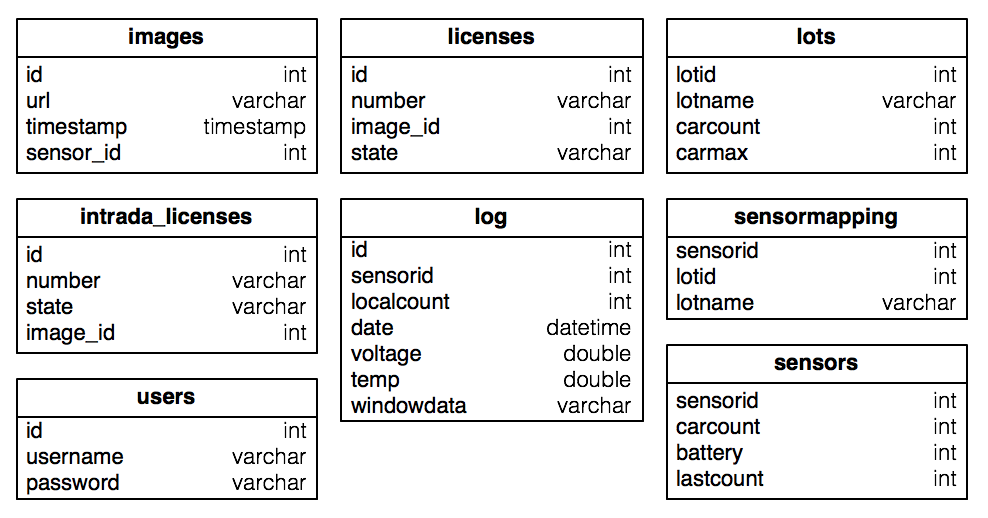
\includegraphics[width=5in]{schema}
\end{center}
\caption{MySQL Database Schema}
\label{fig:schema}
\end{figure}

\subsubsection{Administrator Website}
Much of the work done on the ACMx server during this project involved developing and deploying the administrator website. The site serves as an easy-to-use interface that provides tools for administrators (our group members and ACMx group members). These tools allow administrators to view the data collected by the magnetometer sensors and the image-acquisition Raspberry Pis, view health data about the sensors, and manage user accounts. Each component of the administrator website is described below.

\emph{User Account Management}
Administrators are able to create, delete, and view other administrator accounts. Maintaining user accounts is important for this system because our API requires user authentication for certain HTTP routes, as described above. We have created a dedicated user that is allowed to access all the back-end routes; this user is the one that is used by the base station Raspberry Pi to POST its magnetometer and image data to the server. Other administrator accounts are used to gain access to the administrator site, and to provide authentication when testing specific routes.

\emph{License Plate Viewer}
As mentioned in section 2.5, the license plate images are translated by the ALPR software from an image into a string of plain text, and stored in the MySQL database on the ACMx server. One of the main functions of the web interface is to display this data to administrators. The page that displays the license plate data is a simple interface that shows every license plate number we have collected, along with the time it was collected, the parking lot it came from, and the original image that the license number came from. The data is divided into two tables: one for the data returned from the OpenALPR software, and one for the data returned by the Intrada software. The entries are sorted by most-recent first. For this project, we were only interested in creating a proof-of-concept type interface that shows we have the capability to display the collected plate data in a useful format; in the future it could be useful to cross-reference our data with the campus parking department's database to check if a car has entered a lot without a permit.

\emph{Sensor Data Viewer}
Another feature of the administrator webpage is the page that allows administrators to view sensor data. This page maintains a table showing each sensor, its current and last count, its battery level, and the lot where it is deployed. Although this is a simple page, it provides useful information to the administrators of the site. Future additions to this page will include a way to add and remove sensors from the database.

\subsection{Deployment}
{\color{red}\textbf{NOT COMPLETE}}
The system will be deployed at the CTLM Upper and Lower parking lots at CSM. These lots were chosen because of their accessible location, unobstructed visibility from a campus structure, and wide use. Both parking lots have one entryway, each of which will be equipped with an automobile detection subsystem. The junction between the two lots is also of interest, because we want to know when a car moves from the upper lot to the lower lot, and vice versa. The locations of the entrances and junction are shown in Figure \ref{fig:deployment}. The locations for the three sensor nodes benefit from having a clear view of the sky for increased photovoltaic efficiency.
\begin{figure}
\begin{center}
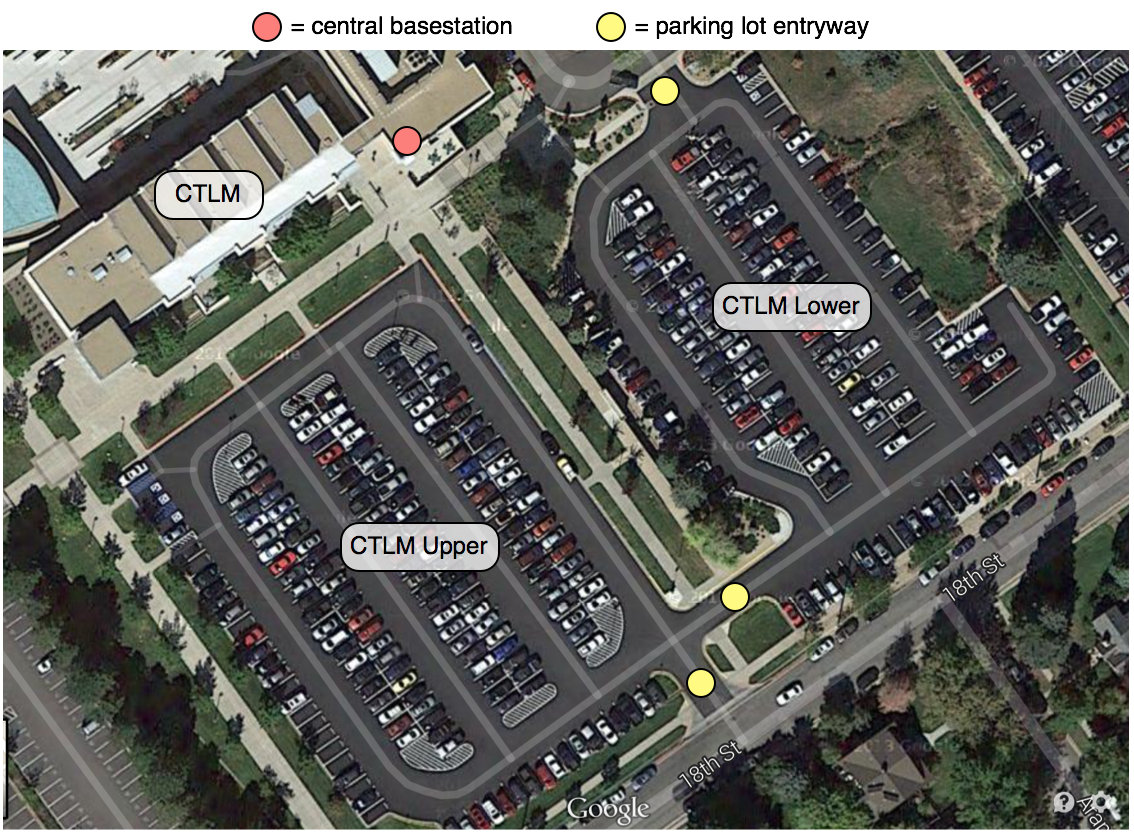
\includegraphics[width=5in]{deployment}
\end{center}
\caption{Deployment Location}
\label{fig:deployment}
\end{figure}

The central base station, as described in section 2.4, will be placed in an upper window of the CTLM building, allowing it to take a clear overhead picture of at least one of the two parking lots. For the first deployment we may only have one overhead camera to start off with, although ideally we would have two - one for each lot. Several potential locations exist which allow for a clear line-of-sight to all automobile detection subsystems, one of which is detailed in Figure \ref{fig:deployment}. The location of the base station must put it in range of the XBees mounted on each sensor node, to allow data to be transferred from the detection subsystem to the base station. The locations being considered must also provide internet access to the base station Raspberry Pi through ethernet ports.

\section{Results}
{\color{red}\textbf{NOT COMPLETE}}


\section{Future Research}

\subsubsection{Validating and Adjusting Lot Capacity Data}
We expect that our first deployment of this system may not be 100\% accurate at detecting all vehicles that enter and exit lots. Therefore, as mentioned in section 2.4, we will be collecting periodic overhead images from a camera mounted on the base station Raspberry Pi. These images will serve as a visual representation of how many cars are actually in the parking lot at the time the image was taken. Administrators should be able to periodically compare this image to the collected data from the sensor network to make sure the numbers being computed by the network accurately represent the number of cars in the lot. The web interface will allow administrators to pull up the image for any lot with an overhead camera and see the numbers for that lot right next to the image. If any discrepancies are found, the administrator should be able to overwrite the count in the database to reflect reality. This interface will be extremely useful in helping to calibrate the system. For example, if the sensors are consistently reporting less cars in the lot than the image shows, we can fine-tune the collection process to make sure fewer cars slip through unnoticed. Future work in this area will include an automated version of this process, where a computer program will compare the image to the sensed data and make any necessary corrections.

\section{Summary}
{\color{red}\textbf{NOT COMPLETE}}
This project extends the work done by ACMx to create the first comprehensive parking management system for the Colorado School of Mines. The proposed expansions cover interfacing with the existing automobile detection network, acquiring images of license plates, processing those images, and presenting the resulting data in a web application.

Acquiring images of license plates will include experimentally testing the timing of taking the picture, as well as on-mote pre-processing of the image. By completing some processing of the image on the Raspberry Pi, we can both reduce the size of data we need to transmit (saving battery power), while also avoiding transmitting false positives (when no license plate is detected).

Image acquisition will come from several acquisition Raspberry Pis stationed at parking lot entrances. These images will be sent to a central base station, which will then upload the data to a server. Once on the server, additional image processing will be done to retrieve the characters composing the license plate. This data will be stored in a database for use in the web application.

In addition, the base station Raspberry Pi will sample images of the parking lots to allow administrators to correct the status of the system. This may happen when the acquisition motes unsuccessfully identify a car entering or exiting, and therefore have incorrect information regarding the parking lot's capacity.

The web application will serve to show the state of the parking lots, as well as offer a way for administrators to reconcile observed data (from base station images) and sensed data (from acquisition motes). Administrators will also be able to access license plate data from processed images to show proof-of-concept for this utility.

Once deployed, the SmartLots system, augmented with our additional license plate extraction subsystem and improvements to the web application, will offer the Mines campus an accessible way to manage campus parking lots. Faculty and students will be able to use this to find open parking and save time. Future applications could include interfacing with Parking Services to locate illegally parked vehicles or to gather data regarding campus parking needs.


\begin{thebibliography}{99}
\bibitem{stillwell2013} R. Stillwell, A. Wilson ``Magnetometer Parking Sensor,'' \emph{EGGN 383 Final Project, Colorado School of Mines}. December 12, 2013.

\bibitem{parkingWiki} R. Stillwell. (2014). \emph{Parking Sensor Wiki} [Online]. Available: \url{http://github.com/ColoradoSchoolOfMines/parking_sensor/wiki}

\bibitem{openCV} \emph{OpenCV} [Online] Available: \url{http://opencv.org/}

\bibitem{raspbian} \emph{Raspbian} [Online] Available: \url{http://www.raspbian.org/}

\bibitem{REST} \emph{Representational State Transfer} [Online] Available: \url{http://en.wikipedia.org/wiki/Representational_state_transfer}

\bibitem{Slim} \emph{Slim} [Online] Avaliable: \url{http://www.slimframework.com/}

\bibitem{du2013} S. Du et. al., ``Automatic License Plate Recognition (ALPR): A State-of-the-Art Review,'' \emph{IEEE Trans. Circuits and Systems for Video Technology}, vol. 23, no. 2, Feb. 2013.

\bibitem{intrada2014} Q-Free ASA. (2014). \emph{OCR Technology} [Online]. Available: \url{http://www.q-free.com/product/ocr-technology/}

\bibitem{patel2012} C. Patel et al., ``Optical Character Recognition by Open Source OCR Tool Tesseract: A Case Study,'' \emph{Intl. Journal Computer Applications} vol. 55, no. 10, Oct. 2012.

\end{thebibliography}


\section*{Appendix 1 --- Intrateam Work Distribution}


\section*{Appendix 2 --- Code Listings}
\subsection*{Arduino Fio Sensing Firmware}
\begin{spacing}{1}
\begin{lstlisting}[language=java]
/*
Arduino, HMC5883, magnetometer, XBee code 
 by: Roy Stillwell, Andrew Wilson
 Colorado School of Mines
 created on: 10.30.13
 license: This work is licensed under a Creative Commons Attribution license.
 updated: 3.19.14 Roy Stillwell
 updated: 4.25.14 Santiago Gonzalez
 
 Arduino code example for interfacing with the HMC5883 
 by: Jordan McConnell
 SparkFun Electronics
 created on: 6/30/11
 license: OSHW 1.0, http://freedomdefined.org/OSHW
 
 Analog input 4 I2C SDA
 Analog input 5 I2C SCL
 
 EEPROM code adapted from Tomorrow Lab
 Developer: Ted Ullricis_measuringh <ted@tomorrow-lab.com>
 http://tomorrow-lab.com
 
 
 ******************
 HOW IT WORKS:
 ******************
 
 An array of 'baseline' or nominal values -essentially when the sensor does NOT have a vehicle over it- is gathered initially. 
 This baseline can be 'sized' to allow for fine tuning using the 'baselineSize' variable in the 'Variables you can change' section.
 After the initial buffer is filled, its average is calculated. 
 A sensor value is then read and compared to the average and a threshold.  If it is outside this threshold, a counter is started.  
 Once The counter is larger than the window size ( a very good indication of a car), we have detected a vehicle! 
 We then grab the last three values in the window and check to see if it is greater or smaller than the baseline average.  
 This gives us a direction of the vehicle.  
 
 The code <will be> designed to re-calibrate the 'baseline' every 10 minutes (basically in the event a sensor is hit wiht a solar storm or something).
 
 Currently this only uses the Y axis data (as that may be all we need)
 Using datasets taken at the CTLM exits and entrances, it correctly calculates entrances and exits.
 
 */

#include <Wire.h> //I2C Arduino Library, required for interface communication with HMC5883 Device
#include "stats.h"  //a custom library for doing Average and Standard deviation calculations.
#include <cmath>  //Standard cmath library
#include <string>
using namespace std;
#include <avr/wdt.h>
#include <avr/sleep.h>
#include <avr/interrupt.h>



//----------Variables you can change--------------------
double recalibrateTime = 600000; //time in seconds. 600000 = 10 min -- used to auto-recalibrate sensor, if time is greater than 10 minutes, recalibrate
#define baselineSize 100  //Size of baseline to use for baseline values
#define windowSize 30  //Size of 'window' to use for previous values of the sensor to be considered in calculating a positive detection.
#define windowConsidered 3 //Consider the first n numbers in window to determine direction
double carThreshold = 15.0; //Used to sort out car 'hits'. Anything above or below this 'threshold' is counted as a hit
double pingTime = 60; //(in seconds) Used to make sure sensor is still alive after specified time
//------------------------------------------------------


const int battPin = A0;
const int ledPin = 13;
const int interruptPin = 12;
const int XBeeSleep = 2;               // Connect to XBee DTR for hibernation mode
const int waitPeriod = 1;              // Number of 8 second cycles before waking
// up XBee and sending data (8*8 = 64 seconds)
// Variable Definition

//double Vcc = 0.0;
double Temp = 0.0;
double batt = 0.0;

double pingCounter;    //Used to count cycles so system can 'ping' basestation every 30 seconds
int localCarCount=0;
long startTime ;                    // start time for the algorithm watch
long elapsedTime ;                  // elapsed time for the algorithm
bool didWeCalculateAveDevAlready, saidit = false;
double lastCalibrateTime, stdDev;
double baselineAvg = 0;
double calibrationPercentDone;
int x, y, z;
int windowTotal = 0, count = 0, detectorCount = 0;
int baseline[baselineSize];
int windowy[windowSize];
int windowx[windowSize];
int windowz[windowSize];
String yomama_data;


#define address 0x1E //0011110b, I2C 7bit address of HMC5883

String getWindowData(int window[]) {
  String data = "";
 for (int i = 0; i < windowSize; i++ ) {
   data+= String(window[i]) + " ";
 }
 return data;
}
  

// See: http://code.google.com/p/tinkerit/wiki/SecretVoltmeter
//double readVcc() {
//  signed long resultVcc;
//  double resultVccFloat;
//  // Read 1.1V reference against AVcc
//  ADMUX = _BV(REFS0) | _BV(MUX3) | _BV(MUX2) | _BV(MUX1);
//  delay(10);                           // Wait for Vref to settle
//  ADCSRA |= _BV(ADSC);                 // Convert
//  while (bit_is_set(ADCSRA,ADSC));
//  resultVcc = ADCL;
//  resultVcc |= ADCH<<8;
//  resultVcc = 1126400L / resultVcc;    // Back-calculate AVcc in mV
//  resultVccFloat = (double) resultVcc / 1000.0; // Convert to Float
//  return resultVccFloat;
//}

// See: http://code.google.com/p/tinkerit/wiki/SecretThermometer
double readTemp() {
  signed long resultTemp;
  double resultTempFloat;
  // Read temperature sensor against 1.1V reference
  ADMUX = _BV(REFS1) | _BV(REFS0) | _BV(MUX3);
  delay(10);                           // Wait for Vref to settle
  ADCSRA |= _BV(ADSC);                 // Convert
  while (bit_is_set(ADCSRA,ADSC));
  resultTemp = ADCL;
  resultTemp |= ADCH<<8;
  resultTempFloat = (double) resultTemp * 0.9338 - 312.7; // Apply calibration correction (Roy S)
  resultTempFloat = resultTempFloat * 1.8 + 32.0;  // Convert to F
  return resultTempFloat;
}

double readBatt() {
  batt = analogRead(battPin) * .00324 * 2 ;
  return batt;
}

void configureSensor() {
  Wire.begin(); //Initalize I2C interface in Arduino

  //Put the HMC5883 IC into the correct operating mode
  Wire.beginTransmission(address); //open communication with HMC5883
  Wire.write(0x02); //select mode register
  Wire.write(0x00); //continuous measurement mode
  Wire.endTransmission();

  //Crank the speed up to 75Hz read speeds (default is 15Hz)
  Wire.beginTransmission(address);
  Wire.write((byte) 0x00);
  Wire.write((byte) 0x18); //this jumps it to 75Hz
  Wire.endTransmission();
  delay(5);

  //Tell the HMC5883 where to begin reading data
  Wire.beginTransmission(address);
  Wire.write(0x03); //select register 3, X MSB register
  Wire.endTransmission();

  //Read data from each axis, 2 registers per axis (helps initialize readings)
  Wire.requestFrom(address, 6);
  if(6<=Wire.available()){
    x = Wire.read()<<8; //X msb
    x |= Wire.read(); //X lsb
    z = Wire.read()<<8; //Z msb
    z |= Wire.read(); //Z lsb
    y = Wire.read()<<8; //Y msb
    y |= Wire.read(); //Y lsb
  }
  //Pause 
  delay(1000);

}

void setup(){
  //Initialize Serial speed
  Serial.begin(57600);
  configureSensor();
  
  pinMode(interruptPin, OUTPUT); 
  digitalWrite(interruptPin, HIGH); 
  
  Serial.print("You have 10 seconds to place sensor");
  delay(10000);
  

}

//The main loop to repeat indefinitely
void loop(){

  //Tell the HMC5883 where to begin reading data
  Wire.beginTransmission(address);
  Wire.write(0x03); //select register 3, X MSB register
  Wire.endTransmission();


  //Read data from each axis, 2 registers per axis
  Wire.requestFrom(address, 6);
  if(6<=Wire.available()){
    x = Wire.read()<<8; //X msb
    x |= Wire.read(); //X lsb
    z = Wire.read()<<8; //Z msb
    z |= Wire.read(); //Z lsb
    y = Wire.read()<<8; //Y msb
    y |= Wire.read(); //Y lsb
  }
  
  //Get temp and voltage data
  //Vcc = (double) readVcc();
  Temp = (double) readTemp(); 
  batt = (double) readBatt();
  

  //build the baseline array to be used for average calculation
  if (count < baselineSize) {
    baseline[count] = y;
    if (count == 0) {
      Serial.println("Calibrating...");
    }
      //Echo out to serial how far we are in calibrating.
      //    double calibrationPercentDone =  baselineSize;
      //    calibrationPercentDone = count / calibrationPercentDone * 100;
      //    Serial.print("Hang on, Calibrating ");
      //    Serial.print(calibrationPercentDone);
      //    Serial.print("% done. ");
      //    Serial.print(x);
      //    Serial.print(" ");
      //    Serial.print(y);
      //    Serial.print(" ");
      //    Serial.println(z);

      delay(40);  //Pause for a bunch of cycles so the values are collected over a few seconds.
      count++; //increment counter to fill buffer of size 'baselineSize'
      
      if (count==baselineSize) {
        Serial.println("Done. Ready to take data.");
      }
    }

  

  //Figure out baseline values
  if (count == baselineSize && didWeCalculateAveDevAlready == false) {  //The baseline array is full, so we can begin collecting data!
    baselineAvg = Average(baseline); //get average
    
    didWeCalculateAveDevAlready = true;
    startTime = millis(); 
  }

//  elapsedTime = millis() - startTime;
//  //TODO: write recalibration code
//  if (elapsedTime > recalibrateTime) {
//    //look to recalibrate by building a new temp array
//
//    //check standard deviation of new array against current standard deviation
//    //if within limits, use the new calibration data
//    Serial.println("Uh hang on a minute, recalibrating.");
//    startTime = millis();
//    count = 0;
//  }


  bool something = false;  //used to flag whether or not something is over the sensor

  //This algorithm calculates whether 'something' was found, and then to be sure, starts a detectorCount to verify
  //there are enough hits to constitute an actual car passing, and not some random flux in the Earth's field.
  if ( didWeCalculateAveDevAlready == true && (y >= (baselineAvg + carThreshold) || y <= (baselineAvg - carThreshold))) {
//    Serial.print("[something here ");
//    Serial.print(y);
//     Serial.println("]");
    something = true;  //something is probably out there!

    delay(14); //The HMC is set to run at 75Hz, this delays just that amount!

    //When 'something' may be out there, there are three scenarios.  
    //1) The detector count goes up if there are less 'something' hits than the window size,
    //2) The detector count hits the windows size -what we qualify as a true car over the sensor!- and as such reports it,
    //3) There wasn't a new event, and the detector count is decremented.  Once it hits zero, the car is thought to have passed the sensor
    // Effectively, while a car is over the sensor, detectorCount stops counting, and sort of cruises at the max window size.  As the car passes
    //and sensor values drop to the nominal baseline, it starts clearing the detectorCount buffer and readies for a new car.

    // 1) Something may be in the works, we need to count the 'something' events to be sure and store it in the window
    // We will use the detectorCount as the indexer
    if (detectorCount <= windowSize) {
      windowy[detectorCount] = y;  //We add the current value to the window, for analysis later
      windowx[detectorCount] = x;
      windowz[detectorCount] = z;
    }
    detectorCount++;  

    if (detectorCount >= windowSize && saidit==false) { //here we check to see if we have detected enough events
      //We did detect a car! Now to see direction
      double windowAve;

      for (int i=0; i < windowConsidered; i++) { //using the first few values of the window (the orignal direction of the Magfield)
        //we find the direction.
        windowAve += windowy[i]; //add up all the values
      }
      windowAve = windowAve / windowConsidered;  //generate the average value to be used

        //If the first value is less than the average, we have a car heading in! So transmit!
      if (windowAve < baselineAvg  ) {
        localCarCount++;   
      
        String windowData = getWindowData(windowy);
        Serial.print("<");
        Serial.print(localCarCount); //output car count
        Serial.print(" ");
        //Serial.print(Vcc); //output battery voltage (in theory)
        //Serial.print(" ");
        Serial.print(batt);
        Serial.print(" ");
        Serial.print(Temp); //output device temp (in theory)
        Serial.print(" ");
        Serial.print(windowData);
        Serial.println(">");
        
        //TODO Calibrate temp
        //TODO verify vcc output is correct NOTE, it wasn't. went to new 'batt' calculation


        digitalWrite(interruptPin, LOW); // send interrupt to Raspberry Pi 
        delay(500);
        digitalWrite(interruptPin, HIGH);
        pingCounter = 0; // Device has communicated with the base station, so reset counter for communication
      } 
      else {  //Otherwise the car was heading out!
        localCarCount--;

        //The data packet will automatically be split into 'frames' by the xbee 
        //so we will 'encpauslate' our data. ex: < data > .
        String windowData = getWindowData(windowy);
        Serial.print("<");
        Serial.print(localCarCount); //output car count
        Serial.print(" ");
        //Serial.print(Vcc); //output battery voltage (in theory)
        //Serial.print(" ");
        Serial.print(batt);
        Serial.print(" ");
        Serial.print(Temp); //output device temp (in theory)
        Serial.print(" ");
        Serial.print(windowData);
        Serial.println(">");
        
        //TODO Calibrate temp
        //TODO verify vcc output is correct

        //Serial.print ("Data: ");
        digitalWrite(interruptPin, LOW); // send interrupt to Raspberry Pi 
        delay(500);
        digitalWrite(interruptPin, HIGH);
        pingCounter = 0; // Device has communicated with the base station, so reset counter for communication
      }
      //For debugging, we echo the window average and baseline average to makes sure the algorithm is working
      //        Serial.print("windowAve: ");
      //        Serial.print(windowAve);
      //        Serial.print(" baselineAvg: ");
      //        Serial.println (baselineAvg);
      saidit = true; //mark that we have said there is a car already, so we don't repeat it
    }

  } 
  else {
        //3) An event was not detected, so the detectorCount begins decrementing its values
            if (detectorCount > 0) detectorCount--;
            //Once it zero, the algorithm is essentially ready for a new car.
            if (detectorCount == 0) saidit = false;
        
            //This code does is used for diagnostics.  It essentially sends a 'heartbeat' to the base station
            if (pingCounter >= (pingTime*200)) { // is about 1 second with this program code 
              //To be sure everything is working (mostly for diagnostics, ping every 30 seconds).
                    //The data packet will automatically be split into 'frames' by the xbee 
        
        //so we will 'encpauslate' our data. ex: < data > .
        String windowData = getWindowData(windowy);
        Serial.print("<");
        Serial.print(localCarCount); //output car count
        Serial.print(" ");
        //Serial.print(Vcc); //output battery voltage (in theory)
        //Serial.print(" ");
        Serial.print(batt);
        Serial.print(" ");
        Serial.print(Temp); //output device temp (in theory)
        Serial.print(" ");
        Serial.print(windowData);
        Serial.println(">");
              pingCounter = 0;
              //delay(40);
         }
         pingCounter++;  
  }

}
\end{lstlisting}
\end{spacing}

\subsection*{ALPR Invocation Function}
\begin{spacing}{1}
\begin{lstlisting}[language=php]
function get_license_number($image_filepath, $image_url) {
	$license_number = "FAIL";
	$intrada_license_number = "FAIL";
	$state = NULL;

	// Start the OpenALPR engine on the ACMx server.
	// Sample result string (plate is LTM378):
	// - LTM378 confident: 92.4582 template_match: 0
	$unfiltered_result = exec("/var/license_plates/openalpr/src/alpr -r /var/license_plates/openalpr/runtime_data -n 1 $image_filepath");

	if ($unfiltered_result != '') {
		$exploded_result = explode(' ', $unfiltered_result);
		$license_number = $exploded_result[5];
	}

	// Create a SOAP request for Intrada ALPR cloud service.
	$intrada_client = new SoapClient('http://intrada2.cloudapp.net/IntradaService.asmx?WSDL',
		array('soap_version' => SOAP_1_2));
	$intrada_request = $intrada_client->IntradaRecognizeDirectPassage(
		array(
			'project' => 'brodrigu.demo',
			'key' => '8053',
			'images' => array($image_url),
			'metadata' => array()
		)
	);

	// Sample result string (plate is LTM378):
	// RESULT:{hash}:{plate},{confidence},{state},{confidence},{coordinates of license plate in image}:{execution time}
	// RESULT:592E1EE8D1DE427BB6E0042F34745523:LTM378,750,USA_CO,750,(309,156),(503,159),(309,206),(503,207):1594
	$unfiltered_result = $intrada_request->IntradaRecognizeDirectPassageResult;
	if (!is_soap_fault($unfiltered_result)) {
		$exploded_result = explode(':', $unfiltered_result);
		$unfiltered_result = $exploded_result[2];
		if ($unfiltered_result == '[reject]' || $unfiltered_result == 'Could not download file') {
			$unfiltered_result = 'REJECT';
		}
		$exploded_result = explode(',', $unfiltered_result);
		$intrada_license_number = $exploded_result[0];
		if ($unfiltered_result != 'REJECT') {
			$state = $exploded_result[2];
		}
	}

	// $license_number will be FAIL if OpenALPR didn't find a number, or the plate/partial.
	// $intrada_license_number will be FAIL if Intrada had an error,
	// [reject] if it could not find a number, or the plate/partial.
	$license_info = array(
		0 => $license_number,
		1 => $intrada_license_number,
		2 => $state
	);

	return $license_info;
}
\end{lstlisting}
\end{spacing}


\end{document}  
